\documentclass{article}

\usepackage[preprint]{neurips_2025}
\usepackage[utf8]{inputenc}
\usepackage[T1]{fontenc}
\usepackage{amsmath}
\usepackage{amssymb}
\usepackage{booktabs}
\usepackage{float}
\usepackage{graphicx}
\usepackage{hyperref}
\usepackage{microtype}
\hypersetup{hidelinks}

\title{High-Dimensional Arrhythmia Classification from Raw ECG Time Series with Spectral and Random-Matrix Analysis}
\author{%
  ECG RMT Analysis \\
  ML 7501 Applied Machine Learning
}

\newcommand{\R}{\mathbb{R}}
\newcommand{\AUC}{\operatorname{AUC}}

\begin{document}
\maketitle

\begin{abstract}
This work studies binary arrhythmia screening from raw PTB-XL electrocardiogram waveforms using engineered time--frequency features and random-matrix diagnostics. Each ECG is decoded from WFDB files, mapped through SCP diagnostic statements, featurized across the twelve leads, and evaluated on the official PTB-XL folds. The final design matrix contains 17,084 training records and 594 preprocessed columns after imputation, scaling, and one-hot encoding. Six classifier families are compared under the same fold protocol: regularized logistic regression, a stochastic linear margin model, random forest, extremely randomized trees, histogram gradient boosting, and XGBoost. XGBoost obtains the highest held-out test ROC-AUC, 0.9097, while histogram gradient boosting obtains the highest test F1, 0.8378. Random Matrix Theory is not used as a classifier. Instead, it is used to measure the high-dimensional geometry of the feature matrix and to stress-test fitted models. The standardized covariance spectrum has aspect ratio \(p/n=0.0348\), Marchenko--Pastur support \([0.662,1.408]\), and 60 eigenvalues above the upper edge, explaining 76.9\% of variance. Re-evaluating trained models on MP-outlier and MP-bulk reconstructions shows that the predictive score functions are largely preserved by outlier components and strongly degraded in the bulk. A separate retraining experiment with MP filtering and PCA++ positive pairs from ECG half-segments did not improve held-out accuracy or ROC-AUC over original XGBoost. The final conclusion is that RMT is a useful diagnostic for this feature map, but hard spectral filtering is not a performance improvement.
\end{abstract}

\section{Introduction}

High-dimensional ECG classification is not only a supervised learning problem; it is also a question about whether a large feature basis contains stable diagnostic structure or mostly estimation noise. PTB-XL provides ten-second, twelve-lead ECGs with expert SCP-ECG statements. A standard applied pipeline can decode the waveforms, construct labels, extract features, and train classifiers. That pipeline is necessary but not sufficient for understanding model behavior in a regime where hundreds of engineered variables are learned from a finite cohort.

This project therefore uses Random Matrix Theory (RMT) as a diagnostic layer. The Marchenko--Pastur (MP) law gives a null reference for eigenvalues of a high-dimensional covariance matrix under independent noise. Components above the MP upper edge are treated as structured outliers, while components inside the MP support form the empirical bulk. The central question is whether the trained ECG classifiers obtain their discrimination from the outlier subspace or whether the MP bulk is also carrying substantial predictive signal.

The contribution is empirical and methodological: a reproducible PTB-XL binary classification pipeline is combined with a model-level RMT stress test. The analysis reports ordinary held-out metrics and, separately, how each fitted model behaves when its test inputs are reconstructed from MP-outlier versus MP-bulk principal components. This keeps RMT in the role of spectral analysis, not as an extra competing classifier.

\section{Data, Labels, and Feature Map}

Let \(r_i\in\R^{T\times L}\) be the decoded waveform for record \(i\), with \(L=12\) ECG leads and \(T=1000\) samples for the 100 Hz PTB-XL files used here. Let \(q_i\) denote the row of recording metadata. PTB-XL stores a dictionary of SCP statement likelihoods; after joining those codes to \texttt{scp\_statements.csv}, let \(C_i\) be the set of mapped diagnostic superclass labels for record \(i\). The binary target is
\begin{equation}
  y_i =
  \begin{cases}
    0, & C_i=\{\mathrm{NORM}\},\\
    1, & \exists c\in C_i: c\ne \mathrm{NORM}.
  \end{cases}
  \label{eq:target}
\end{equation}
Records with no mapped diagnostic superclass are removed from supervised modeling. This leaves 21,388 labeled records from 21,799 metadata rows. The retained records contain 9,069 normal labels and 12,319 diagnostic-abnormality labels. At the diagnostic-superclass level, the mapped counts are \texttt{NORM}: 9,514, myocardial infarction: 5,469, ST/T change: 5,235, conduction disturbance: 4,898, and hypertrophy: 2,649. These counts exceed the number of records because PTB-XL records can carry multiple diagnostic statements. The resulting binary task is therefore a screening abstraction over a multi-label clinical annotation scheme rather than a replacement for subclass diagnosis.

The raw feature map is
\begin{equation}
  z_i=\phi(r_i,q_i)\in\R^{p_0},\qquad p_0=523.
\end{equation}
The map contains per-lead time-domain statistics, derivative statistics, band-power and FFT descriptors, cross-lead correlations, and selected metadata fields. The time-domain block includes amplitude moments, quantiles, interquartile range, root-mean-square amplitude, energy, skewness, kurtosis, derivative moments, and zero-crossing rate. The frequency-domain block is computed from the real FFT and includes total spectral power, spectral centroid, dominant frequency, spectral entropy, roll-off frequencies, band powers, and band fractions. Cross-lead correlations are included because morphology changes can appear as coordinated lead patterns rather than isolated univariate effects.

Preprocessing is fitted only on the training folds. For numerical feature \(j\), the transform is
\begin{equation}
  \tilde{x}_{ij}
  =
  \frac{\operatorname{impute}(z_{ij};\operatorname{median}_{\mathrm{train},j})-\mu_{\mathrm{train},j}}
  {s_{\mathrm{train},j}},
  \label{eq:preprocess}
\end{equation}
where \(\mu_{\mathrm{train},j}\) and \(s_{\mathrm{train},j}\) are computed after imputation on the training folds. Categorical metadata fields are most-frequent imputed on the training folds and then one-hot encoded with unseen validation/test levels ignored. This avoids using validation or test statistics during preprocessing. Metadata missingness was nonuniform: height was missing for 67.7\% of modeling records, weight for 56.2\%, nurse identifier for 6.7\%, and site for 0.07\%. In contrast, decoded waveform feature missingness was negligible, with the largest signal-feature missing fraction below 0.005\%. The final preprocessed vector is \(x_i=g(z_i)\in\R^p\) with \(p=594\) columns after one-hot expansion.

Figure~\ref{fig:preprocessing} gives the preprocessing diagnostics used before model selection. The class prevalence is stable across the official train, validation, and test folds: the abnormal fraction is 57.6\%, 57.4\%, and 57.7\%, respectively. The constructed target is also associated with age: normal records have median age 54 years (IQR 40--65), while diagnostic-abnormality records have median age 67 years (IQR 57--76). This difference is not used as a clinical claim; it is a cohort shift that the models must handle under fold-preserving evaluation. Among engineered waveform variables, cross-lead correlations have the largest mean absolute univariate association with the target, followed by global signal descriptors and lead-level spectral features. The top individual correlations remain moderate, with the largest \(|\rho|=0.382\) for the correlation between leads I and aVF.

\begin{figure}[H]
  \centering
  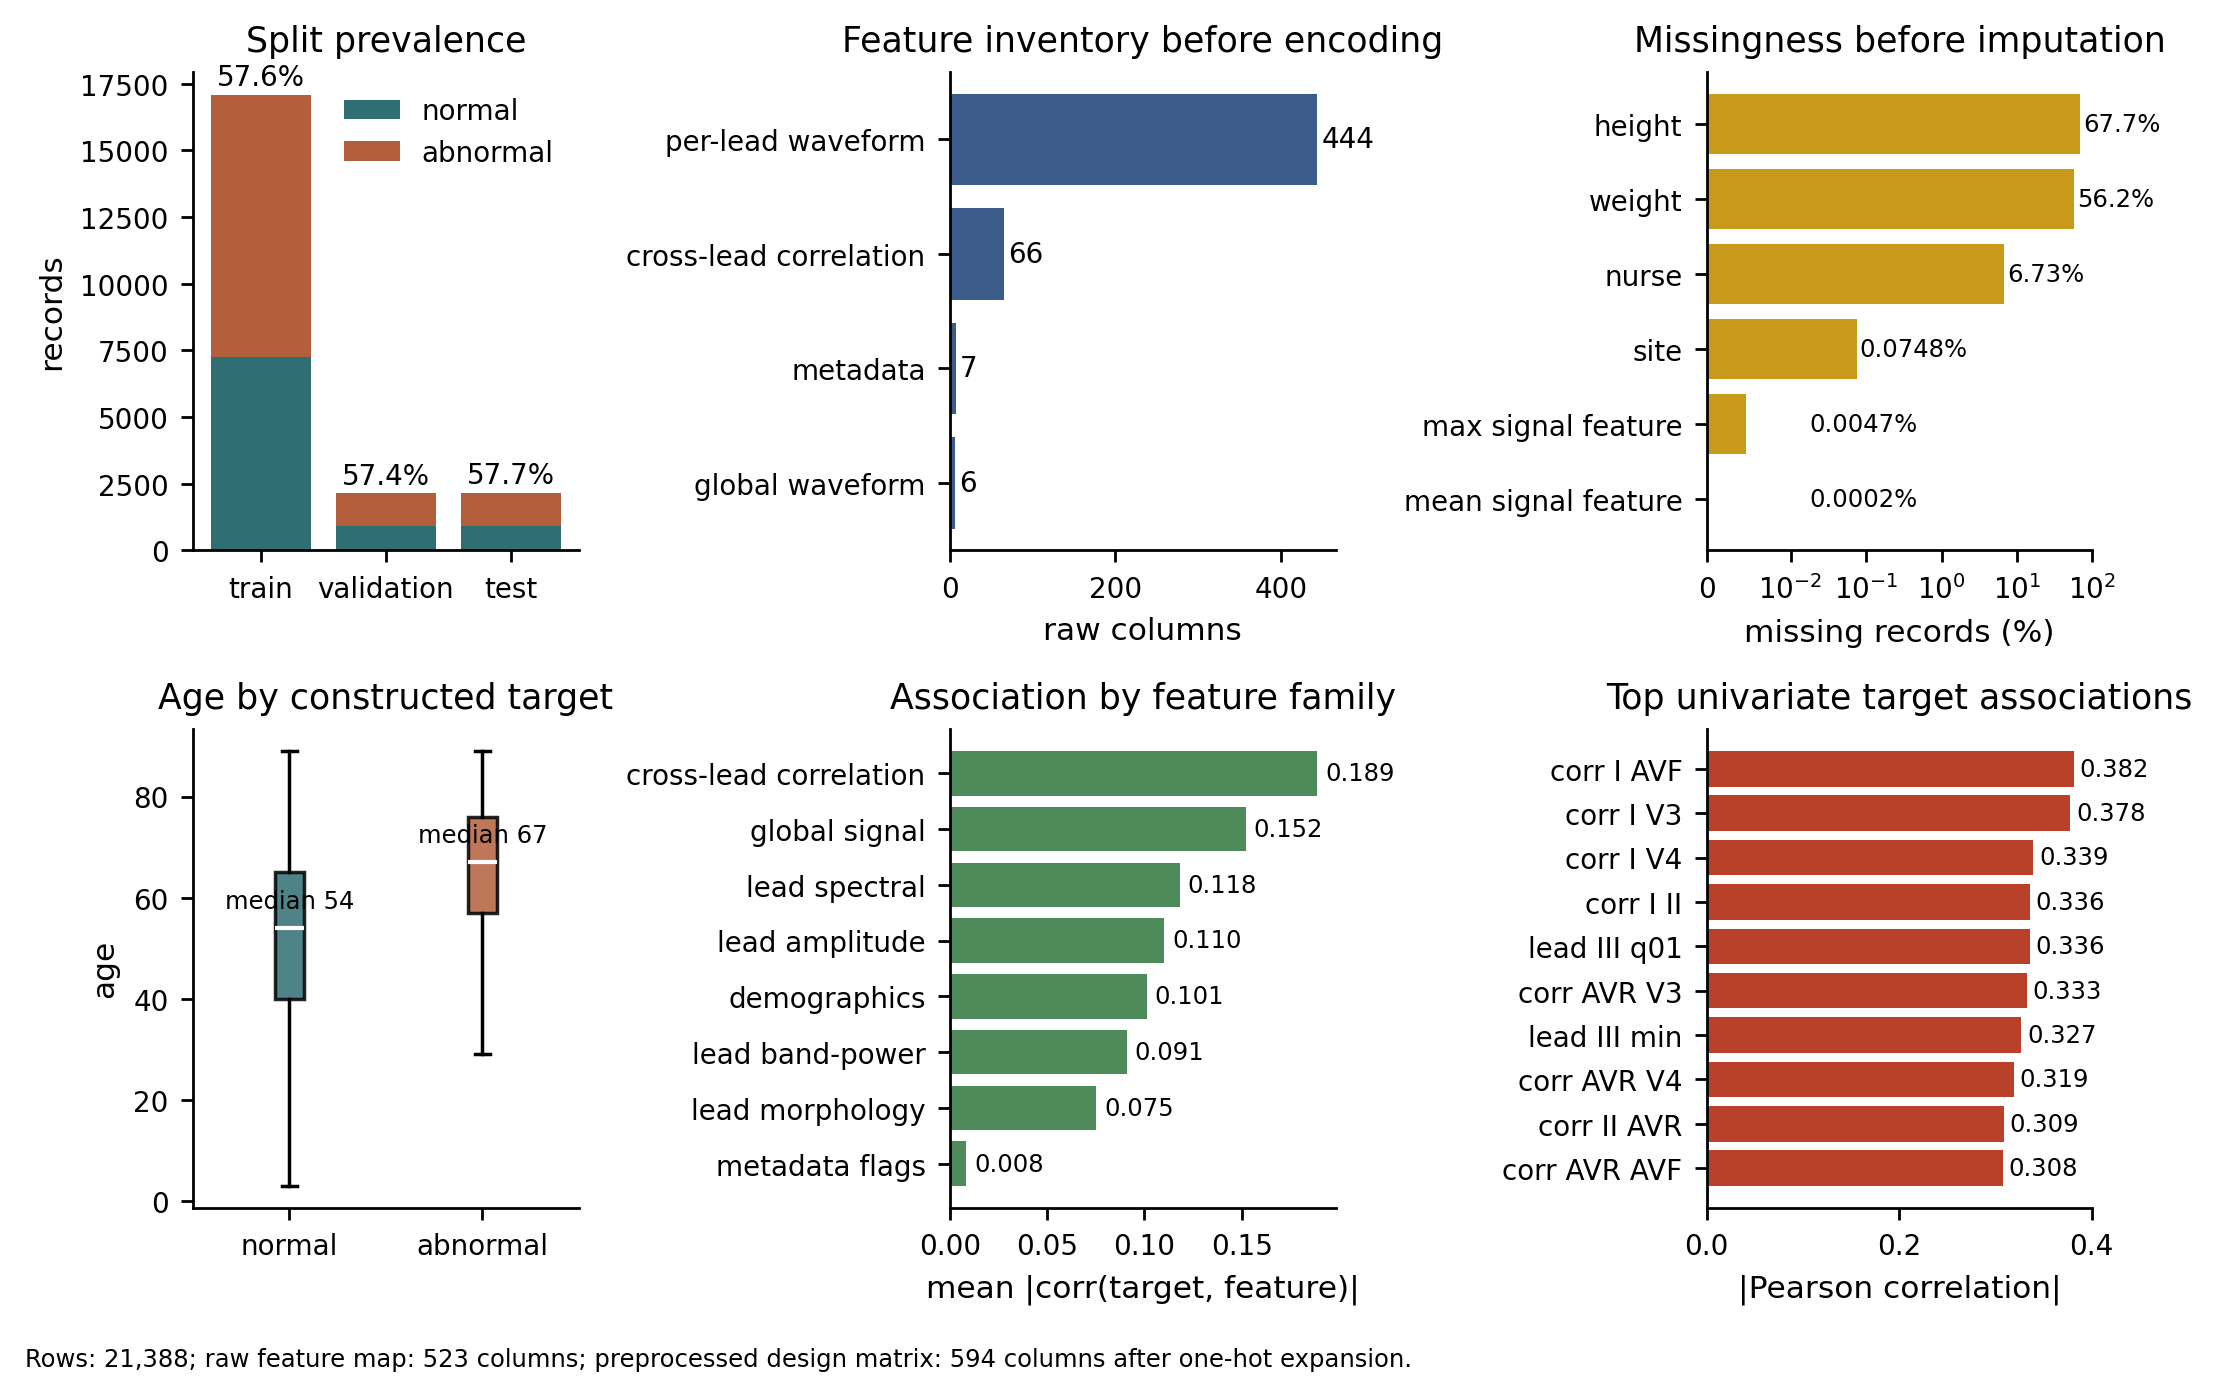
\includegraphics[width=\linewidth]{figures/paper_preprocessing_findings.png}
  \caption{Preprocessing and feature-quality diagnostics from the row-level Modal modeling table. A: target prevalence by official fold split. B: raw feature inventory before categorical one-hot expansion. C: missingness before imputation. D: age distribution by constructed binary target. E: mean absolute target correlation aggregated by feature family. F: strongest individual absolute Pearson correlations with the target.}
  \label{fig:preprocessing}
\end{figure}

The official PTB-XL folds are preserved: folds 1--8 are used for fitting and cross-validation, fold 9 for validation, and fold 10 for final testing. Table~\ref{tab:split} gives the supervised split.

\begin{table}[H]
  \centering
  \caption{Supervised dataset split from the official PTB-XL folds.}
  \label{tab:split}
  \begin{tabular}{lrrr}
    \toprule
    Split & Normal & Diagnostic abnormality & Total \\
    \midrule
    Train & 7,243 & 9,841 & 17,084 \\
    Validation & 914 & 1,232 & 2,146 \\
    Test & 912 & 1,246 & 2,158 \\
    \bottomrule
  \end{tabular}
\end{table}

\section{Model Selection and Regularization}

For each model family \(m\), the pipeline fits a score function \(f_{m,\lambda}:\R^p\to\R\) with hyperparameters \(\lambda\in\Lambda_m\). Hyperparameters are chosen by stratified cross-validation inside the training folds:
\begin{equation}
  \hat{\lambda}_m=
  \arg\max_{\lambda\in\Lambda_m}
  \frac{1}{K}\sum_{k=1}^{K}
  \AUC\!\left(f_{m,\lambda}^{(-k)}(X_k),y_k\right),
  \qquad K=5.
  \label{eq:optuna}
\end{equation}
The run uses Optuna's TPE sampler with eight completed trials per model. This budget is small enough to report honestly and large enough to compare model families under the same compute envelope. The models cover complementary inductive biases: linear separation with regularization, stochastic high-dimensional margin fitting, bagged trees, randomized trees, histogram gradient boosting, and XGBoost. XGBoost is run in the Modal GPU container with CUDA enabled; the other estimators use CPU parallelism.

The engineered ECG feature map deliberately contains correlated measurements: quantiles correlate with amplitude moments, band fractions correlate with total band power, and homologous leads often move together. For a linear score \(f(x)=\beta^\top x+b\), the regularized empirical objective can be written as
\begin{equation}
  \min_{\beta,b}
  \frac{1}{n}\sum_{i=1}^{n}\ell(y_i,\beta^\top x_i+b)
  +\lambda_1\|\beta\|_1+\frac{\lambda_2}{2}\|\beta\|_2^2.
  \label{eq:regularized-linear}
\end{equation}
The \(L_1\) term encourages sparsity and feature selection by setting many coefficients exactly to zero. The \(L_2\) term shrinks correlated coefficients together and stabilizes estimates under multicollinearity. In this dataset, multicollinearity is expected because features are grouped by lead, frequency band, and summary statistic. The main logistic-regression baseline therefore uses \(L_2\) regularization and tunes \(C=1/\lambda_2\). The stochastic linear model searches both \(L_2\) and elastic-net penalties to test whether sparsity improves the high-dimensional margin model.

\begin{table}[H]
  \centering
  \caption{Selected hyperparameters from Optuna TPE search. The objective is training-set cross-validated ROC-AUC.}
  \label{tab:hyperparams}
  \small
  \begin{tabular}{llp{7.4cm}}
    \toprule
    Model & CV ROC-AUC & Selected setting \\
    \midrule
    Logistic regression & 0.9106 & \(L_2\) penalty with \(C=0.1635\), indicating nontrivial shrinkage rather than an almost unregularized linear fit. \\
    SGD linear & 0.8592 & Modified Huber loss, \(L_2\) penalty, \(\alpha=2.07{\times}10^{-6}\). Elastic-net was searched but not selected. \\
    Random forest & 0.9182 & 400 trees, maximum depth 18, minimum leaf size 2, and 35\% feature subsampling per split. \\
    Extra trees & 0.9159 & 200 trees, maximum depth 18, minimum leaf size 3, and 35\% feature subsampling per split. \\
    Hist. gradient boosting & 0.9311 & Learning rate 0.0209, 350 boosting iterations, 44 leaf nodes, minimum leaf size 48, and \(L_2\) regularization 0.028. \\
    XGBoost & 0.9335 & 600 trees, depth 6, learning rate 0.1124, subsample 0.8478, column subsample 0.8814, min child weight 7.77, \(\lambda=0.302\), \(\alpha=0.0409\). \\
    \bottomrule
  \end{tabular}
\end{table}

The selected settings are consistent with the intended model roles. The linear models use shrinkage to handle correlated engineered features. The forest models restrict depth and require nontrivial leaf sizes to reduce variance. The boosting models use learning-rate, tree-complexity, and explicit regularization parameters to control sequential overfitting; XGBoost's nonzero \(\alpha\) and \(\lambda\) indicate that both sparsity pressure and ridge-style shrinkage were useful in the best boosted-tree configuration.

\section{Random-Matrix Analysis}

Let \(X\in\R^{n\times p}\) be the preprocessed training matrix and let \(\bar{x}\) be its column mean. With centered matrix \(X_c=X-\mathbf{1}\bar{x}^\top\), define the sample covariance
\begin{equation}
  S=\frac{1}{n-1}X_c^\top X_c.
\end{equation}
Let \(d_1\ge\cdots\ge d_p\) be the eigenvalues of \(S\). Under a white-noise null with aspect ratio \(\gamma=p/n\), the MP support is
\begin{equation}
  \lambda_{\pm}=\hat{\sigma}^{2}(1\pm\sqrt{\gamma})^2.
  \label{eq:mp}
\end{equation}
For the standardized covariance plot, \(\hat{\sigma}^{2}=1\), \(n=17{,}084\), \(p=594\), \(\gamma=0.0348\), and therefore \(\lambda_-=0.662\) and \(\lambda_+=1.408\). The outlier index set is
\begin{equation}
  \mathcal{J}=\{j:d_j>\lambda_+\},\qquad
  \mathcal{B}=\{1,\ldots,p\}\setminus\mathcal{J}.
\end{equation}
The empirical spectrum has \(|\mathcal{J}|=60\) outlier components and \(|\mathcal{B}|=534\) bulk components. The outlier components explain 76.9\% of the standardized variance; the spectral effective rank is 84.3. Figure~\ref{fig:data-spectrum} shows both the split/class diagnostics and the MP spectrum.

\begin{figure}[H]
  \centering
  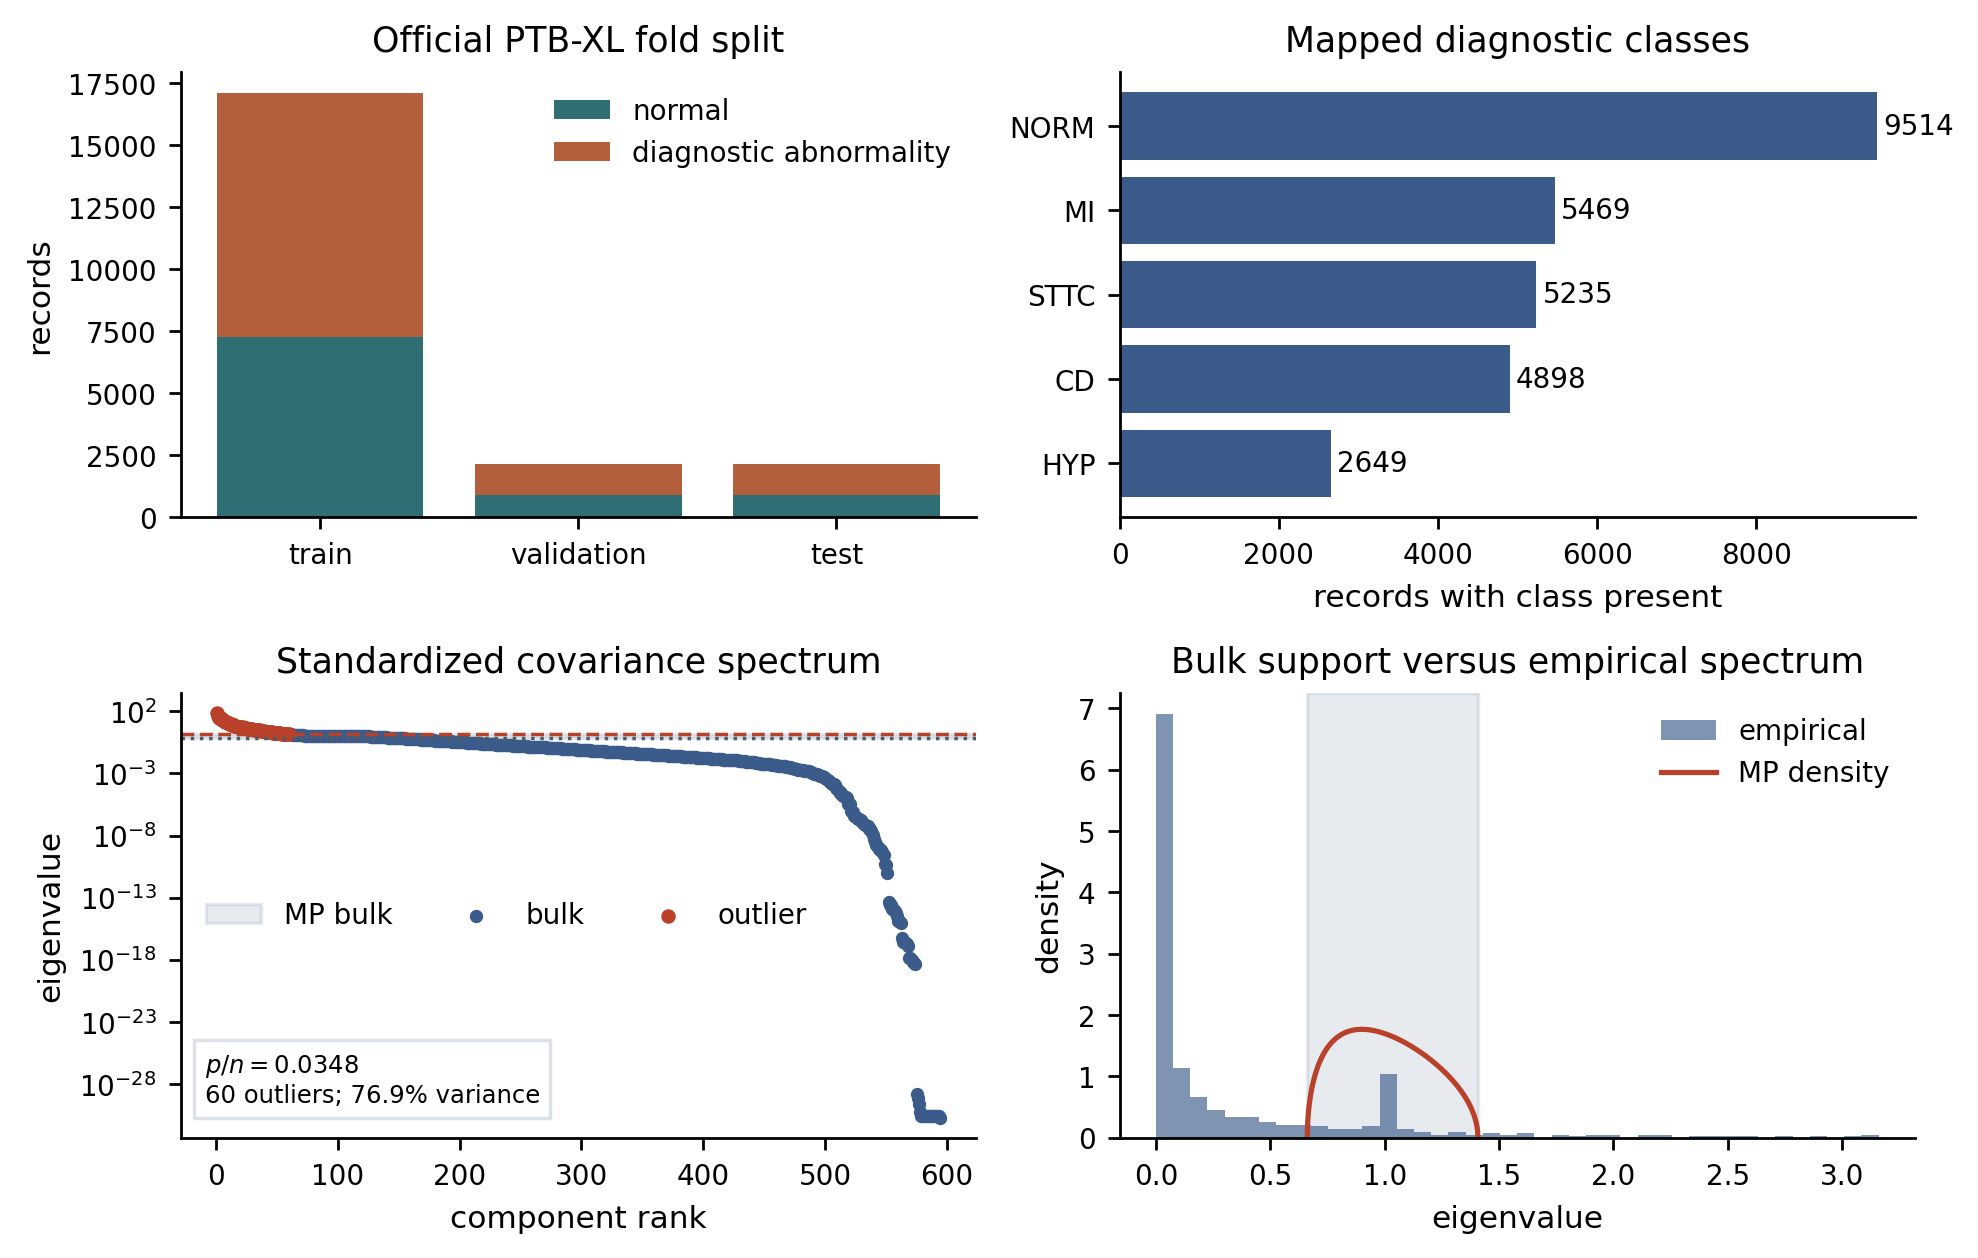
\includegraphics[width=\linewidth]{figures/paper_dataset_spectrum.png}
  \caption{Dataset and covariance-spectrum diagnostics. A: train/validation/test class counts from official PTB-XL folds. B: mapped diagnostic superclass counts. C: eigenvalue spectrum of the standardized training covariance, with MP bulk support shaded and outliers marked. D: empirical eigenvalue histogram near the MP support, overlaid with the MP density.}
  \label{fig:data-spectrum}
\end{figure}

For model behavior, reconstruction is performed in the fitted model-preprocessor basis. In that basis the empirical average eigenvalue is \(\hat{\sigma}^2=0.872\), so the MP support is \([0.577,1.227]\); the selected outlier count remains 60. If \(X_c=U\Sigma V^\top\), define projectors \(P_{\mathcal{J}}=V_{\mathcal{J}}V_{\mathcal{J}}^\top\) and \(P_{\mathcal{B}}=V_{\mathcal{B}}V_{\mathcal{B}}^\top\). For a held-out input \(x\), the two reconstructions are
\begin{equation}
  x_{\mathcal{J}}=\bar{x}+(x-\bar{x})P_{\mathcal{J}},\qquad
  x_{\mathcal{B}}=\bar{x}+(x-\bar{x})P_{\mathcal{B}}.
  \label{eq:reconstruction}
\end{equation}
For each trained model \(f_m\), the diagnostic compares
\[
  \AUC(f_m(X_{\mathrm{test}})),\qquad
  \AUC(f_m(X_{\mathrm{test},\mathcal{J}})),\qquad
  \AUC(f_m(X_{\mathrm{test},\mathcal{B}})).
\]
This is a stress test of the fitted score function. No model is retrained on the reconstructed data, and RMT is not inserted into the classifier pipeline.

Figure~\ref{fig:model-mp} repeats the MP-law view for each model. The ranked spectrum and empirical MP bulk are common across rows because every model is trained from the same preprocessed feature matrix. The model-specific part is the score response in the right column: each row reports the original, MP-outlier, and MP-bulk test ROC-AUC for that fitted model.

\begin{figure}[H]
  \centering
  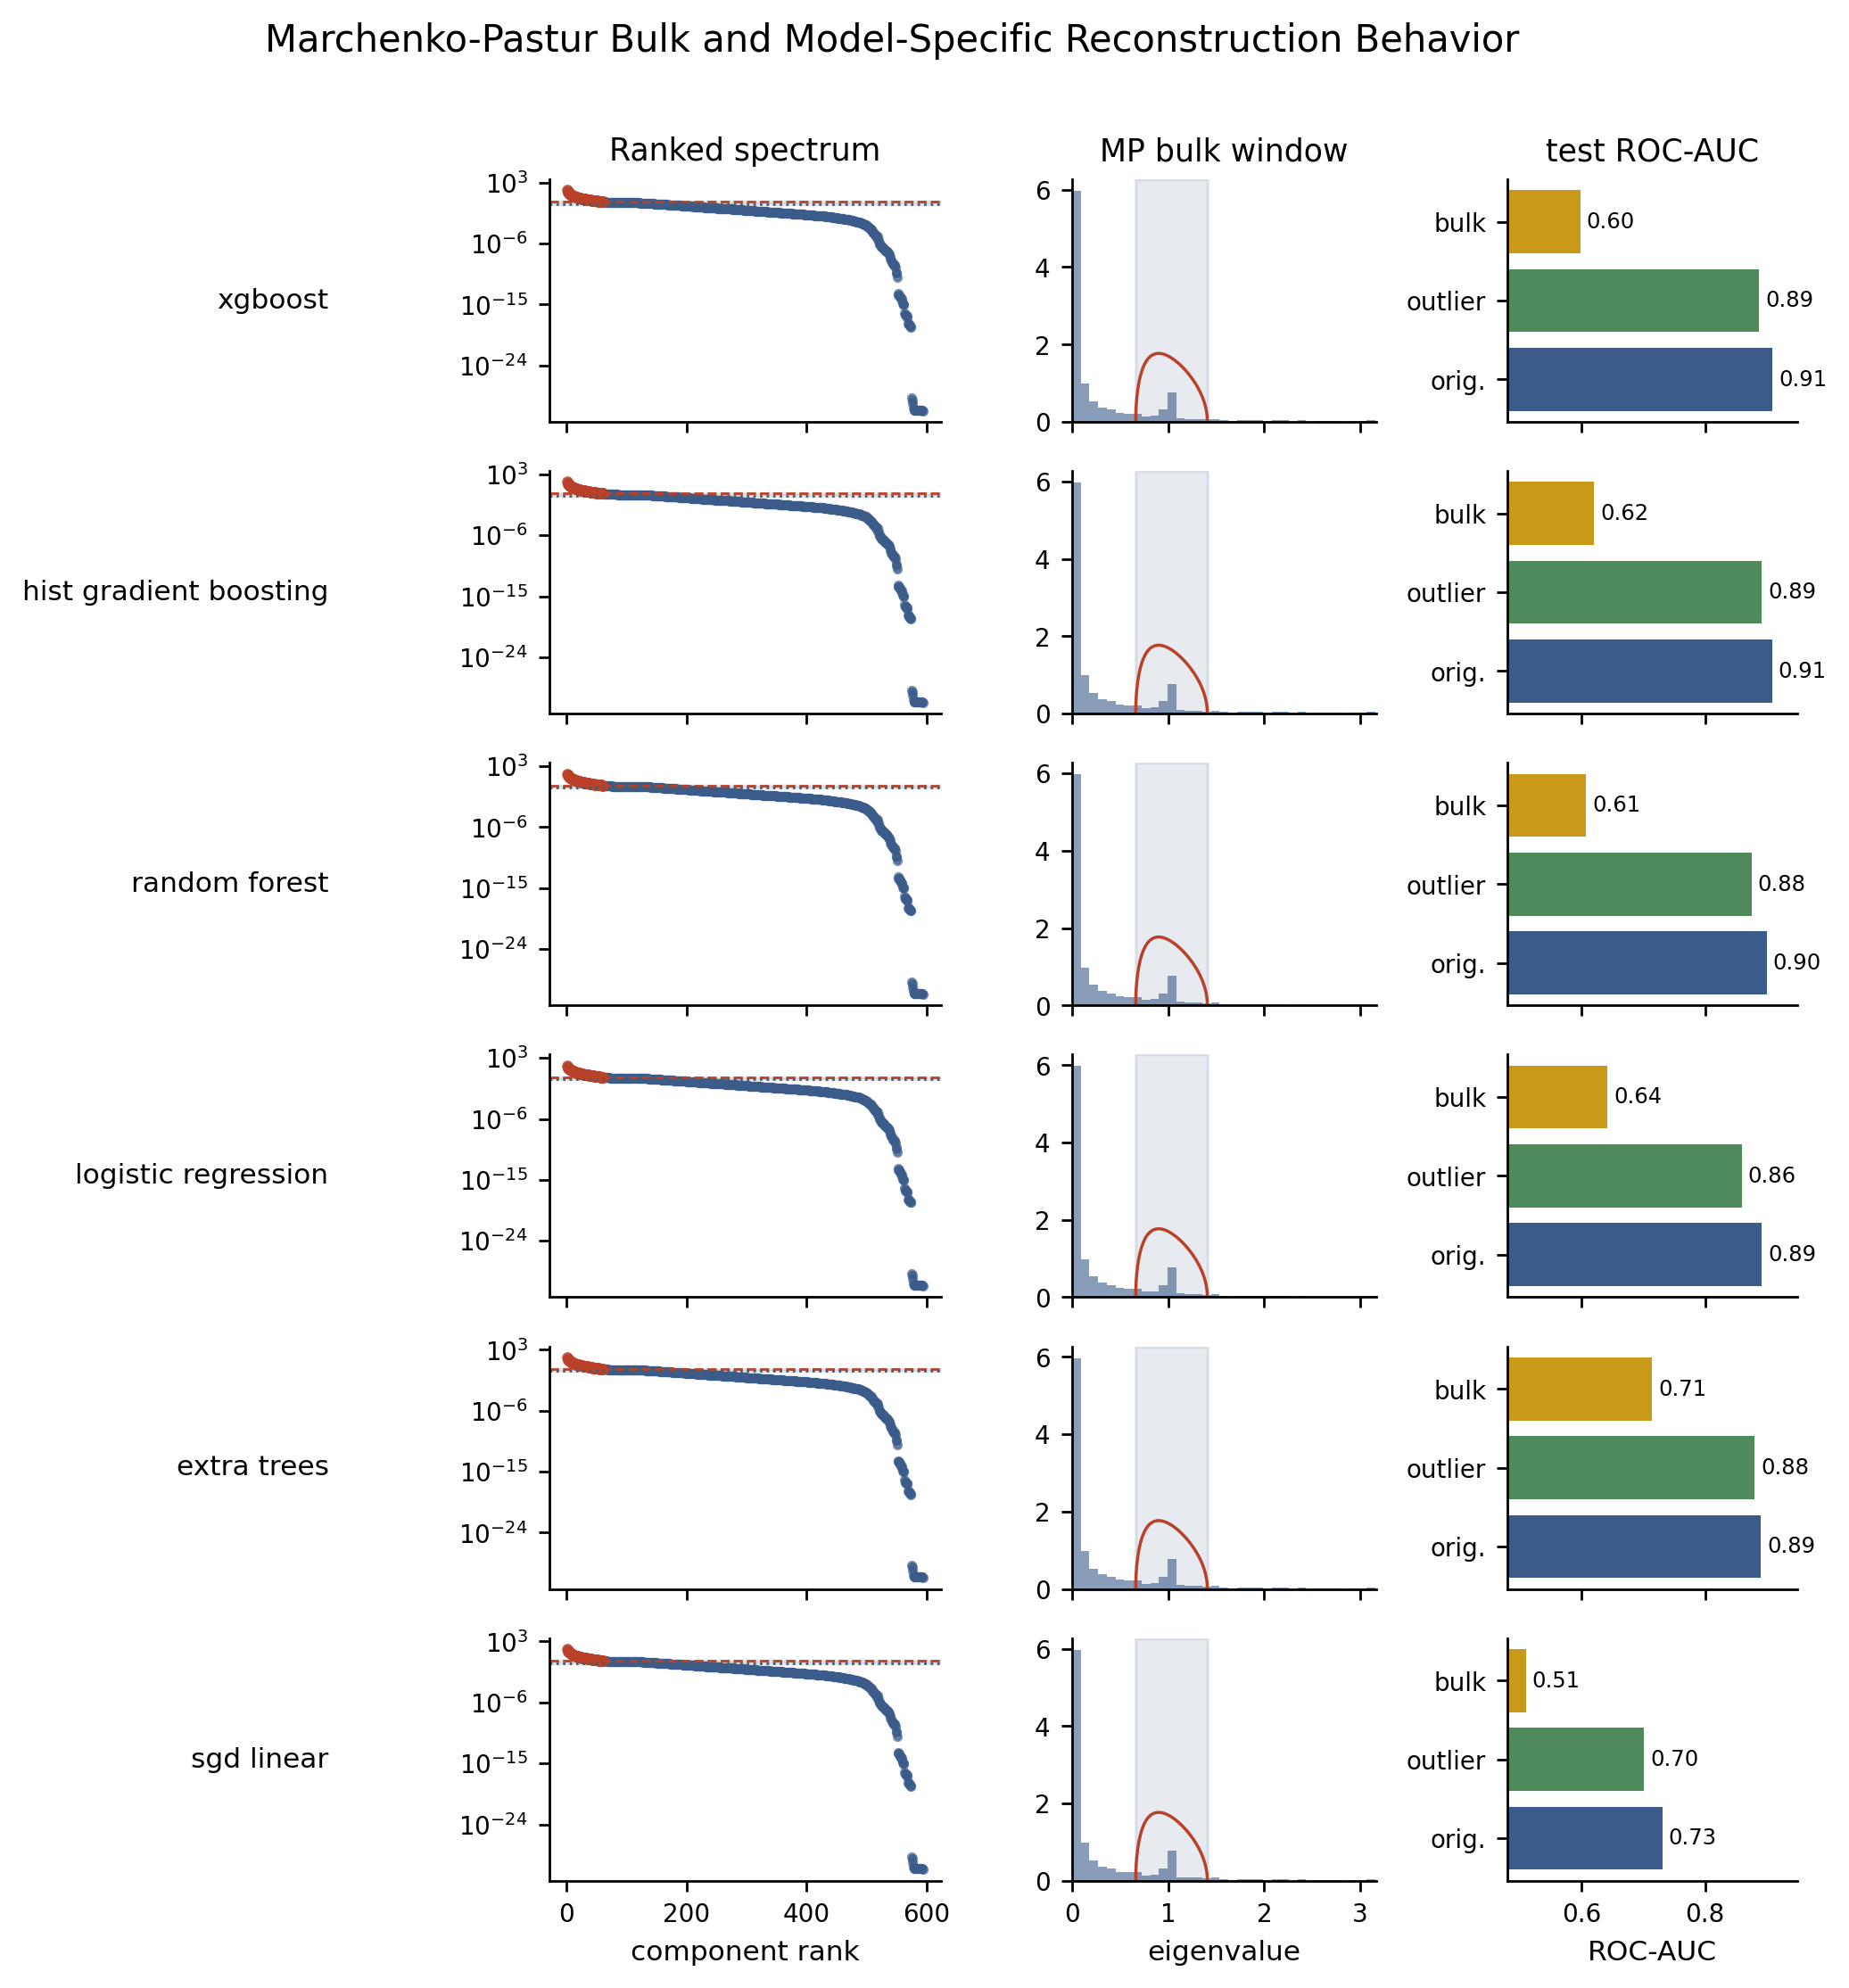
\includegraphics[width=\linewidth]{figures/paper_model_mp_law_facets.png}
  \caption{Per-model Marchenko--Pastur analysis. Each row shows the same spectral decomposition of the preprocessed training matrix and the corresponding fitted model's test ROC-AUC under original inputs, MP-outlier reconstructions, and MP-bulk reconstructions.}
  \label{fig:model-mp}
\end{figure}

\section{Bulk Removal and Bias--Variance Interpretation}

The previous RMT diagnostic probes fitted score functions but does not answer whether removing the MP bulk improves a retrained classifier. To test that claim directly, the validation-selected best model family, XGBoost, is retrained on three signal-filtered representations. The first is the MP outlier score map
\begin{equation}
  h_{\mathcal{J}}(x)=(x-\bar{x})V_{\mathcal{J}}\in\R^{60},
\end{equation}
which removes all 534 bulk coordinates. The second is the MP outlier reconstruction \(x_{\mathcal{J}}\) from Eq.~\eqref{eq:reconstruction}, which keeps the original feature dimension but zeros the bulk subspace. The third follows the PCA++ idea of using ECG half-segment positive pairs: the first and second five-second halves of each training ECG are featurized as paired views, then a generalized eigenproblem selects directions that are stable across the two views. The experiment sets \(k=60\), matching the MP outlier count, and truncates the covariance basis to 99 numerically stable directions above the MP lower edge.

Figure~\ref{fig:rmt-filtering} shows that hard bulk removal did not improve held-out performance. Original XGBoost reached validation/test ROC-AUC 0.9228/0.9097 and test accuracy 0.8151. MP outlier scores fell to test ROC-AUC 0.8839 and accuracy 0.7919. MP reconstruction was the strongest filtered variant, but still reached only 0.8957 test ROC-AUC and 0.8091 accuracy. PCA++ scores from real ECG half-segment positive pairs reached 0.8938 test ROC-AUC and 0.8100 accuracy. The conclusion is negative but informative: the MP bulk is weak when isolated, yet completely removing it discards small complementary information that the original boosted trees can exploit.

\begin{figure}[H]
  \centering
  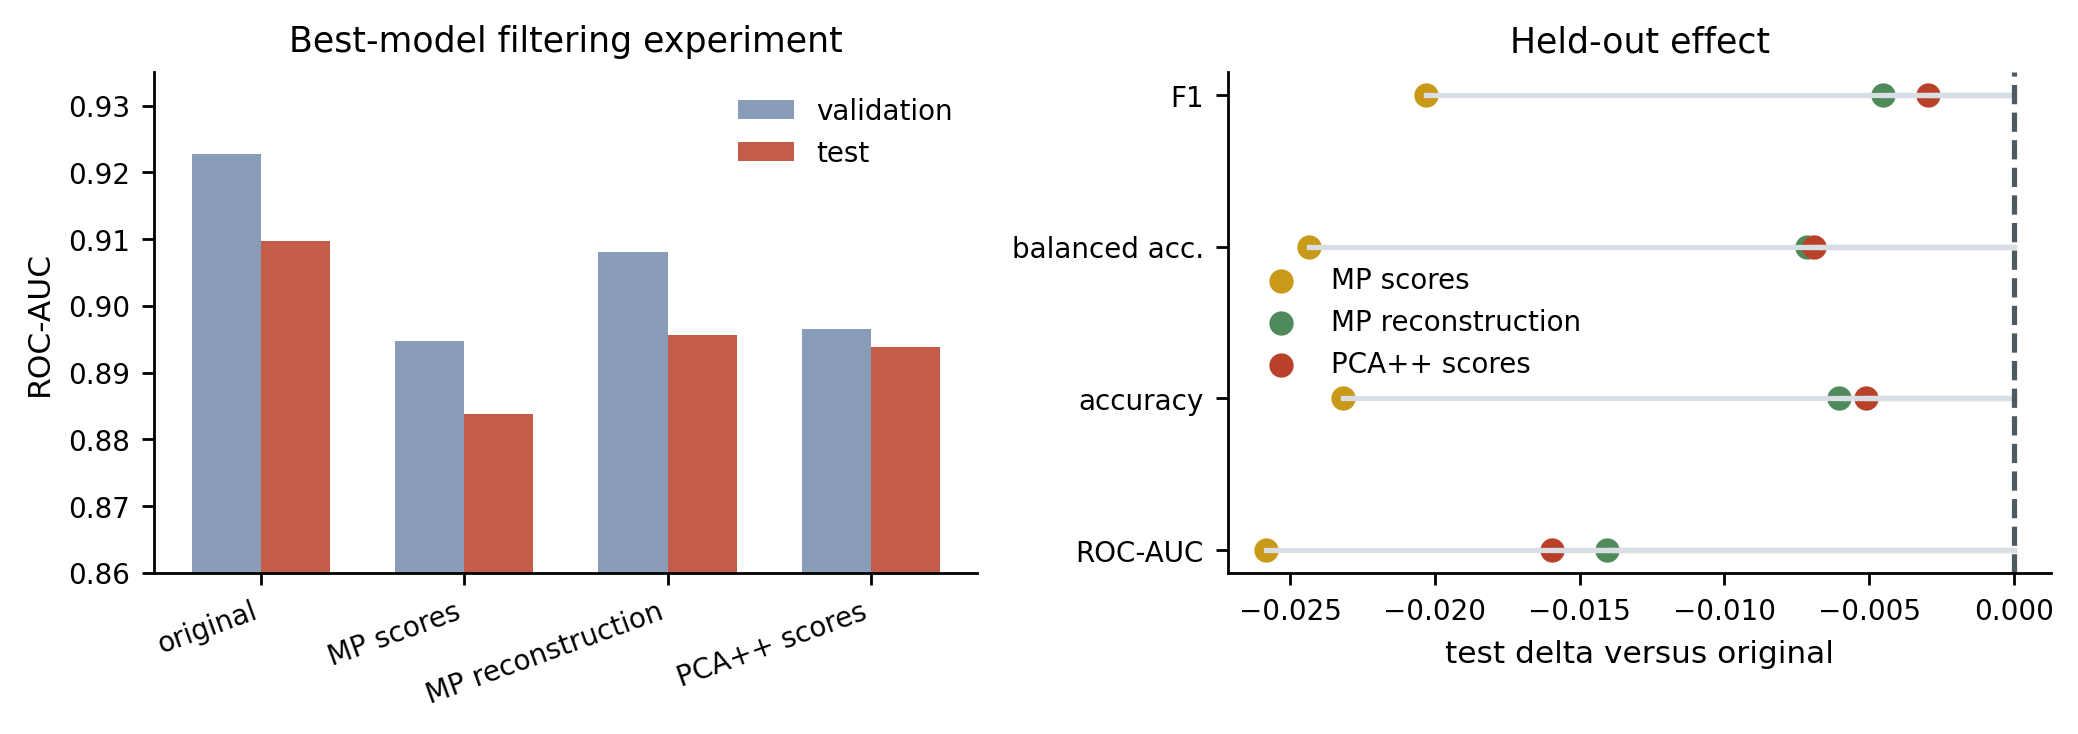
\includegraphics[width=\linewidth]{figures/paper_rmt_filtering_experiment.png}
  \caption{Retraining the validation-selected best model after RMT/PCA++ filtering. A: validation and test ROC-AUC for original XGBoost and three filtered representations. B: held-out test metric changes relative to original XGBoost. None of the filtered representations improves test ROC-AUC or accuracy.}
  \label{fig:rmt-filtering}
\end{figure}

The MP filtering step is mathematically a PCA projection with a data-dependent cutoff. A filtered learner observes \(P_{\mathcal{J}}x\) instead of \(x\), so it searches over a restricted class
\begin{equation}
  \mathcal{F}_{\mathcal{J}}=\{f\circ P_{\mathcal{J}}:f\in\mathcal{F}\}\subseteq\mathcal{F}.
\end{equation}
For a squared-loss surrogate with regression function \(\eta(x)=\mathbb{E}[y\mid x]\), the excess prediction error can be decomposed as
\begin{equation}
  \mathbb{E}\left[(\hat f(P_{\mathcal{J}}x)-\eta(x))^2\right]
  =
  \underbrace{\mathbb{E}\left[(f^*_{\mathcal{J}}(P_{\mathcal{J}}x)-\eta(x))^2\right]}_{\text{approximation bias}}
  +
  \underbrace{\mathbb{E}\left[(\hat f(P_{\mathcal{J}}x)-f^*_{\mathcal{J}}(P_{\mathcal{J}}x))^2\right]}_{\text{estimation variance}}.
\end{equation}
The same qualitative tradeoff applies to the classification scores optimized by logistic, margin, and boosting losses, even though ROC-AUC itself is not a squared-error risk.

For a linear score \(f_\beta(x)=\beta^\top x\), projection is especially restrictive:
\[
  f_\beta(P_{\mathcal{J}}x)=\beta^\top P_{\mathcal{J}}x=(P_{\mathcal{J}}\beta)^\top x,
\]
so the coefficient vector is forced to have no component in \(\operatorname{span}(V_{\mathcal{B}})\). If the best full linear score has \(\beta^*=\beta^*_{\mathcal{J}}+\beta^*_{\mathcal{B}}\), then in the covariance eigenbasis the additional linear approximation error is
\begin{equation}
  \Delta_{\mathrm{bias}}
  =
  (\beta^*_{\mathcal{B}})^\top\Sigma\beta^*_{\mathcal{B}}
  =
  \sum_{j\in\mathcal{B}}d_j(\beta^*_j)^2.
\end{equation}
Thus even small-eigenvalue directions can matter if their coefficients are label-aligned. Removing them lowers estimator variance by reducing the effective dimension, but it increases approximation bias whenever \(\beta^*_{\mathcal{B}}\ne0\). This explains why linear models, already operating with higher approximation bias, are sensitive to outlier-only projection. Tree ensembles have a richer nonlinear hypothesis class and can use threshold interactions in retained high-variance coordinates, so the same projection causes a smaller observed loss. The XGBoost retraining result shows the other side of the tradeoff: although the MP bulk is weak in isolation, it is not pure noise, and hard removal discards enough weak signal to reduce held-out ROC-AUC.

\section{Results}

Table~\ref{tab:test-metrics} reports the final test metrics. XGBoost has the highest test ROC-AUC at 0.9097. Histogram gradient boosting is statistically and operationally close in rank-based performance, with 0.9089 ROC-AUC and the highest F1 at 0.8378. Random forest reaches 0.9001 ROC-AUC. Logistic regression remains competitive at 0.8924, indicating that the engineered features contain strong approximately linear information after preprocessing. SGD is clearly weaker at 0.7307 ROC-AUC.

\begin{table}[H]
  \centering
  \caption{Held-out test metrics from the Modal GPU/Optuna run.}
  \label{tab:test-metrics}
  \small
  \begin{tabular}{lrrrrrr}
    \toprule
    Model & Acc. & Bal. acc. & Prec. & Recall & F1 & ROC-AUC \\
    \midrule
    Logistic regression & 0.7938 & 0.8044 & 0.8877 & 0.7360 & 0.8047 & 0.8924 \\
    SGD linear & 0.7271 & 0.7307 & 0.7973 & 0.7071 & 0.7495 & 0.7307 \\
    Random forest & 0.8100 & 0.8115 & 0.8597 & 0.8018 & 0.8297 & 0.9001 \\
    Extra trees & 0.8021 & 0.8072 & 0.8686 & 0.7745 & 0.8188 & 0.8909 \\
    Hist. gradient boosting & 0.8202 & 0.8231 & 0.8743 & 0.8042 & 0.8378 & 0.9089 \\
    XGBoost & 0.8151 & 0.8183 & 0.8712 & 0.7978 & 0.8328 & 0.9097 \\
    \bottomrule
  \end{tabular}
\end{table}

\begin{figure}[H]
  \centering
  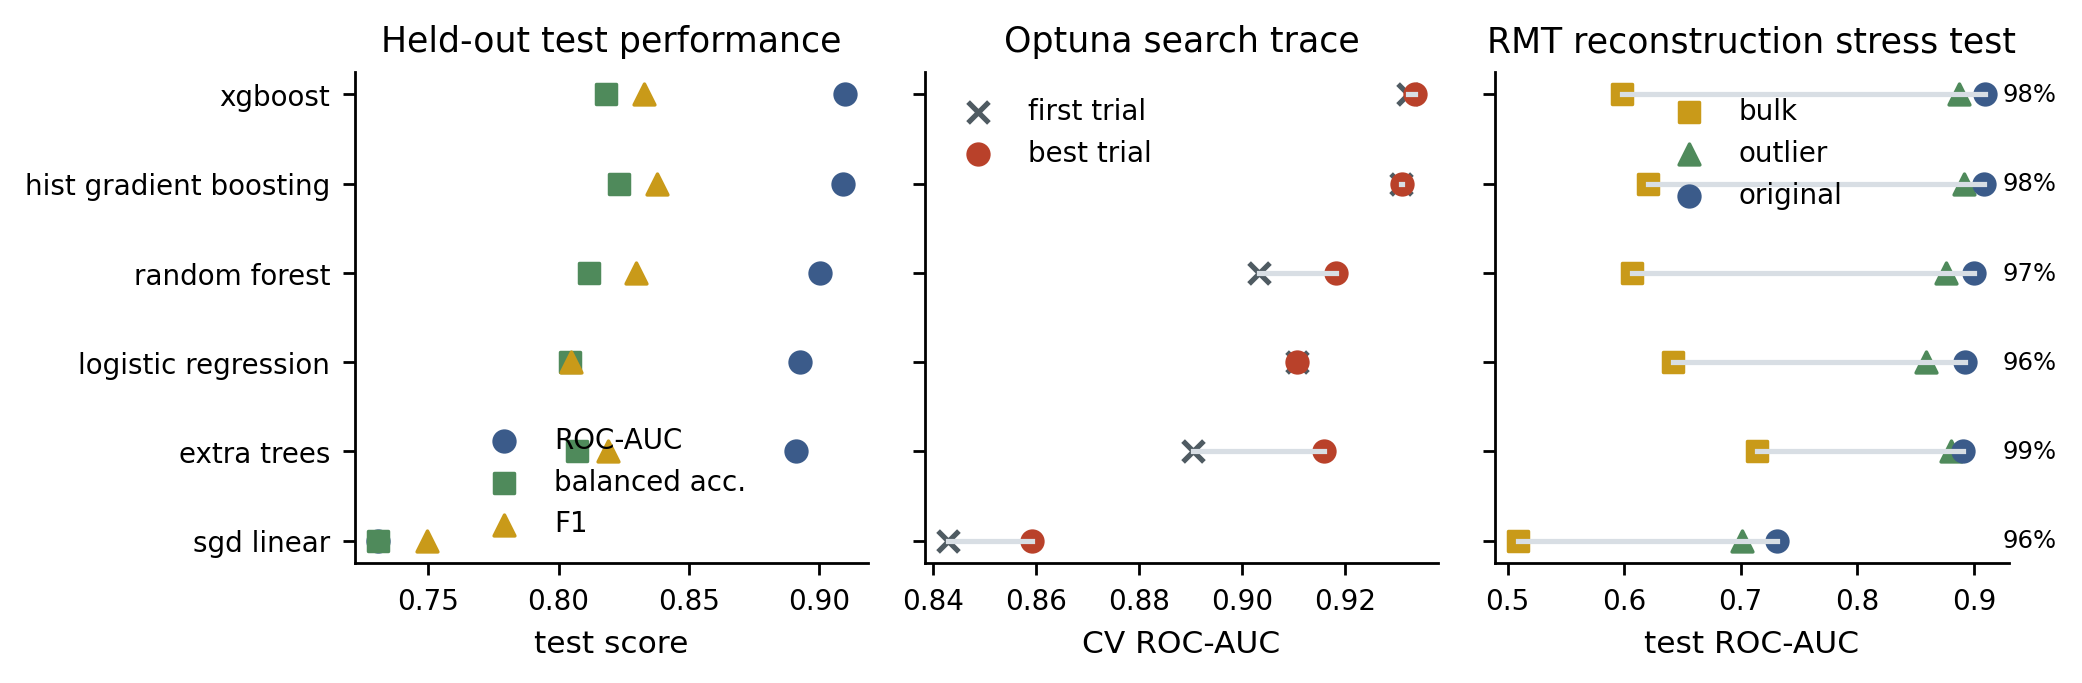
\includegraphics[width=\linewidth]{figures/paper_model_rmt_summary.png}
  \caption{Model comparison and RMT stress test. A: held-out test metrics. B: first versus best Optuna trial, measured by cross-validated ROC-AUC on the training folds. C: original, MP-outlier, and MP-bulk test ROC-AUC for each trained model; right-edge labels give the MP-outlier/original ROC-AUC ratio.}
  \label{fig:model-rmt}
\end{figure}

The RMT stress test gives a sharper explanation of the model rankings than the metric table alone. For XGBoost, test ROC-AUC changes from 0.9097 on original features to 0.8874 on the MP-outlier reconstruction and 0.5979 on the MP-bulk reconstruction. Histogram gradient boosting changes from 0.9089 to 0.8917 and 0.6200. Random forest changes from 0.9001 to 0.8757 and 0.6071. Logistic regression changes from 0.8924 to 0.8592 and 0.6414. These drops are large enough to reject the interpretation that the MP bulk is carrying the main predictive separation.

Extra trees is the exception with the strongest residual bulk behavior: 0.8909 original, 0.8806 outlier-only, and 0.7143 bulk-only ROC-AUC. The bulk score correlation for extra trees is also the highest among the six models, 0.545. This does not make the bulk the dominant signal source, because the outlier reconstruction still preserves 98.8\% of the original ROC-AUC, but it suggests that randomized thresholding can exploit weak residual structure inside the bulk more effectively than the other fitted models. SGD's bulk ROC-AUC is 0.5091, essentially chance, consistent with the overall weakness of that model.

\section{Discussion and Limitations}

The main empirical finding is stable across the best-performing classifiers: MP-outlier reconstructions preserve nearly all rank discrimination, while MP-bulk reconstructions do not. The conclusion is therefore geometric rather than model-specific. The high-dimensional ECG feature matrix has a small dominant subspace relative to its 594 preprocessed columns, and the strongest models use that subspace for most of their discrimination. The retraining experiment adds an important qualification: the MP bulk should not be treated as pure disposable noise for this feature map. Hard removal lowered test performance, which means the bulk contains weak complementary structure even though it is not sufficient on its own.

There are three limitations. First, the binary label in Eq.~\eqref{eq:target} collapses myocardial infarction, ST/T changes, conduction disturbances, hypertrophy, and other abnormal superclasses into one positive class. This makes the screening task tractable but does not solve multi-label ECG interpretation. Second, features are engineered summaries of the raw waveform rather than end-to-end learned representations. Third, the RMT experiment is diagnostic, not causal: projecting onto MP-outlier components tests reliance of fitted score functions, but it does not prove that every outlier direction corresponds to a clinically meaningful mechanism.

Despite these limitations, the experiment satisfies the applied requirement that claims be backed by executed computation on the real PTB-XL data. The code records the data split, preprocessing, model parameters, metrics, RMT spectrum, and reconstruction diagnostics. The reported figures and tables are derived from the saved Modal artifacts.

\section*{References}

\begin{itemize}
\item Akiba, T., Sano, S., Yanase, T., Ohta, T., and Koyama, M. Optuna: A next-generation hyperparameter optimization framework. KDD, 2019.
\item Breiman, L. Random forests. Machine Learning, 2001.
\item Chen, T. and Guestrin, C. XGBoost: A scalable tree boosting system. KDD, 2016.
\item Friedman, J. Greedy function approximation: A gradient boosting machine. Annals of Statistics, 2001.
\item Geurts, P., Ernst, D., and Wehenkel, L. Extremely randomized trees. Machine Learning, 2006.
\item Marchenko, V. and Pastur, L. Distribution of eigenvalues for some sets of random matrices. Mathematics of the USSR-Sbornik, 1967.
\item Pedregosa, F. et al. Scikit-learn: Machine learning in Python. JMLR, 2011.
\item Wagner, P. et al. PTB-XL, a large publicly available electrocardiography dataset. Scientific Data, 2020.
\item Wagner, P. et al. PTB-XL, a large publicly available electrocardiography dataset, version 1.0.3. PhysioNet, 2022.
\item Wu, M., Sun, Q., and Yang, Y. PCA++: How uniformity induces robustness to background noise in contrastive learning, 2025.
\end{itemize}

\end{document}
